\chapter{Interfaz gráfica}
\label{cha:gui}
 
\section{Librerías utilizadas}
Primera sección.
Para el desarrollo de la parte gráfica de este proyecto hemos hecho uso de las librerías:
- PyQt https://www.qt.io/qt-for-python
- Matplotlib
- Pandas
- Seaborn 
 
PyQt
Esta librería está basada en la biblioteca gráfica QT y nos servirá para realizar el diseño de la aplicación    . En nuestro caso optamos por un diseño simple de 2 columnas: En la parte izquierda tendremos los botones y opciones para importar los ficheros de señales y la especificación de la operación, además de un espacio adicional para otras operaciones nuevas a implementar en un futuro. Al lado derecho tendremos la visualización de las señales tratadas y la especificación stl importada.
 
Instalación: 
El desarrollo de la aplicación se hizo en un entorno linux haciendo uso del gestor de paquetes “pip”. 
 
1 - Antes de todo, tenemos que confirmar la versión de Python que tenemos instalada con ´python3 --version´.
 
2 - En el caso de que no lo tuviésemos, instalamos el gestor de paquetes “pip” con sudo ‘apt-get install python3-pip’ y actualizamos el mismo ´pip install -U pip´ 
 
3 - Instalamos la librería PyQT con ´pip install pyqt5´. 
 
\begin{figure}
\centering
  %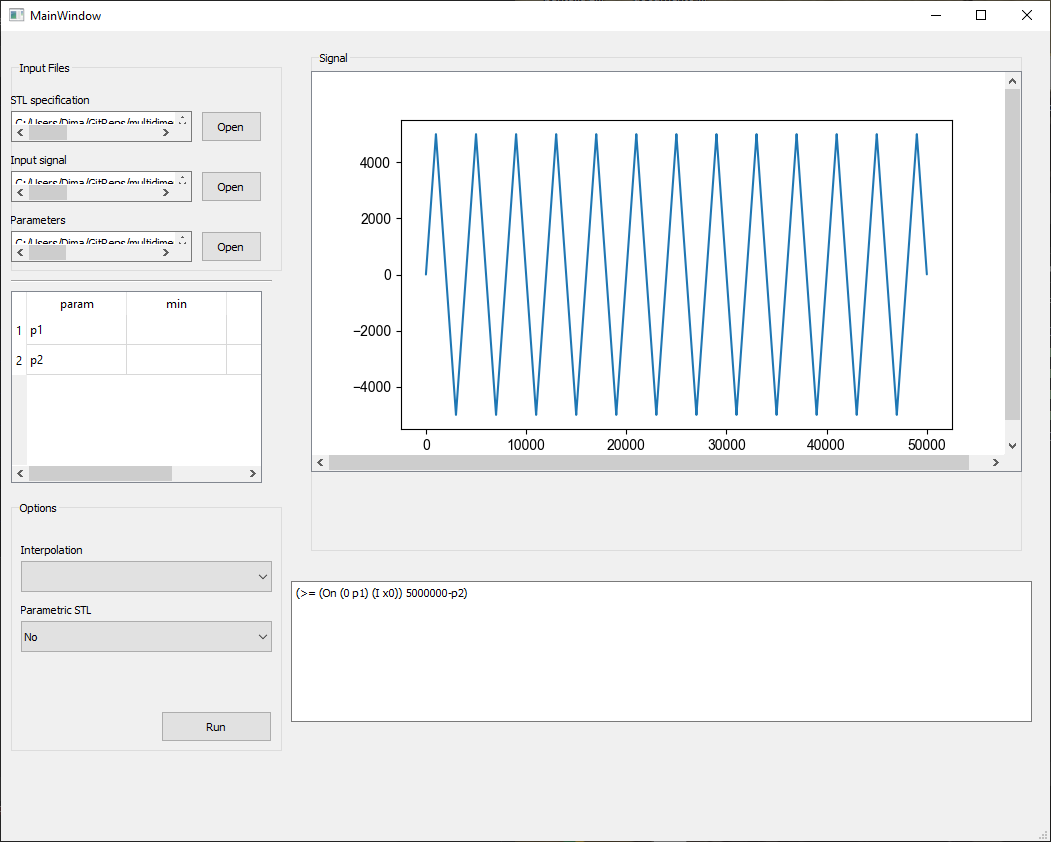
\includegraphics[width=.9\linewidth]{images/gui}
\caption{Nueva pantalla de inicio.}
\label{fig:senal}
\end{figure}
 
MatplotLib
Biblioteca usada para generar gráficos a partir de datos almacenados en un array. Hacemos uso de esta librería con el fin de mostrar las señales resultantes, aplicando las operaciones indicadas, en la sección de la aplicación propuesta para ello. 
 
Instalación: 
 
1 - En este caso es sumamente simple realizando: ´sudo apt-get install python3-matplotlib´.
 
\begin{figure}
\centering
  %\includegraphics[width=.9\linewidth]{images/ejemplo_gui}
\caption{Ejemplo.}
\label{fig:senal}
\end{figure}
 
 
\section{Estructura}
\label{sec:estructura}
La interfaz gráfica, que es completamente novedosa, está montada sobre STLEval y ParetoLib y permite interactuar con ambas herramientas.

La interfaz gráfica permite evaluar tanto expresiones STL estándar (llamadas a STLEval) como minar el rango de validez de fórmulas STL con parámetros (llamadas a ParetoLib).

\begin{figure}
\centering
  %\includegraphics[width=.9\linewidth]{images/diagrama_modulos}
\caption{Señal original y su reconstrucción.}
\label{fig:senal}
\end{figure} 
 
\section{Configuración Técnica}
El tratamiento de las señales se realiza mediante el consumo de la librería ParetoLib y el oráculo de STLe `ParetoLib.Oracle.OracleSTLe`, las funciones más importantes son: 
 
OracleSTLeLib(stl\_prop\_file, csv\_signal\_file, stl\_param\_file): Constructor del objeto basado en la señal de entrada csv, sobre este objeto se van a realizar las operaciones del archivo de especificación que adjuntemos. 
\_load\_stl\_formula(formula): Método que carga un archivo de especificación. 
eval\_stl\_formula(formula): Método que aplica la fórmula anteriormente cargada sobre el objeto `oracle` actual.
 
 
 
 
 
\section{Otros}

